\documentclass[a4paper, 11pt]{article}

\usepackage{xcolor}
\input{/home/aroquemaurel/cours/templates/templates/couleurs.tex}
\usepackage{lmodern}
\usepackage[utf8]{inputenc}
\usepackage[T1]{fontenc} \usepackage[francais]{babel}
\usepackage[top=1.7cm, bottom=1.7cm, left=2.5cm, right=2.5cm]{geometry}
\usepackage{verbatim}
\usepackage{tikz} %Vectoriel
\usepackage{pgfplots}
\usepackage{listings}
\usepackage{fancyhdr}
\usepackage{multido}
\usepackage{amssymb}
\usepackage{multicol}
\usepackage{float}
\usepackage[urlbordercolor={1 1 1}, linkbordercolor={1 1 1}, linkcolor=vert1, urlcolor=bleu, colorlinks=true]{hyperref}

\newcommand{\titre}{Plaquage de textures en lancer de rayons}
\newcommand{\numero}{3}
\newcommand{\typeDoc}{DM}
\newcommand{\module}{Outils Informatiques pour le Multimédia}
\newcommand{\sigle}{OIM}
\newcommand{\semestre}{7}
\newcommand{\auteur}{Antoine de \bsc{Roquemaurel} (G1.1)}

\input{/home/aroquemaurel/cours/templates/templates/classroomsTemplates/l3/tddm.tex}
\input{/home/aroquemaurel/cours/templates/templates/listings.tex} %prise en charge du langage C 
\input{/home/aroquemaurel/cours/templates/templates/classroomsTemplates/l3/remarquesExempleAttention.tex}
\input{/home/aroquemaurel/cours/templates/templates/polices.tex}
\input{/home/aroquemaurel/cours/templates/templates/affichageChapitre.tex}
\makeatother

\begin{document}
	\maketitle
	\section{Avant-propos}
	L'archive que vous avez obtenu sur Moodle contient plusieurs fichiers organisés comme suit : 
	\begin{description}
		\item[\texttt{src/}] Contient uniquement les fichiers modifiés, c'est-à-dire \texttt{main.cpp}, \texttt{texturefetch.cpp} et \texttt{color.hpp}.
		\item[\texttt{images/}] Contient les différentes images produites lors de ce projet
		\item[\texttt{report\_AntoinedeRoquemaurel.pdf}] Le présent rapport que vous êtes en train de lire
	\end{description}

	Comme vous avez pu le voir, j'ai choisi de modifier la classe \texttt{Color}. Ces modifications n'étaient pas indispensables, mais permettait d'améliorer la
	lecture du code. Ainsi j'ai ajouté 3 méthodes : 
	\begin{itemize}
		\item Opérateur \texttt{+=}, permettant d'éviter de faire \texttt{color = color + other}, le \texttt{+=} est plus facile à lire.
		\item De la même manière, l'opérateur \texttt{*=}.
		\item Méthode \texttt{reset()} qui remet toutes les composantes à \texttt{0.f} évitant de créer une nouvelle instance de \texttt{Color}.
	\end{itemize}

	\section{Opérateur \texttt{getTextel()}}
	Une fois les textures intégrés, on peut observer un effet << d'escalier >> sur le quadrillage de l'image, principalement au premier plan, comme le montre la
	figure \ref{fig:fig1}. 

	\begin{figure}[H]
		\centering
		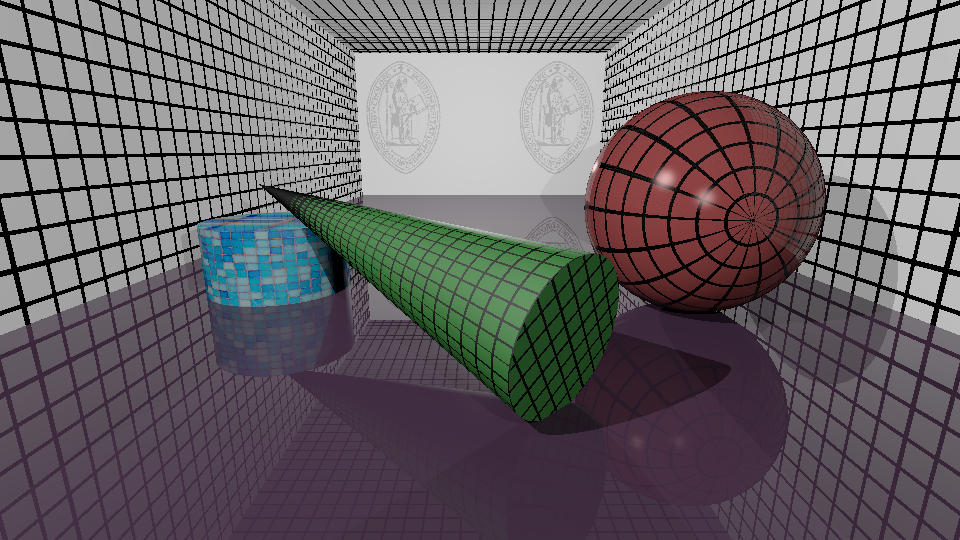
\includegraphics[width=13cm]{images/1-monimage.png}
		\caption{Image obtenue après le développement de \texttt{getTextel()}}
		\label{fig:fig1}
	\end{figure}
	Cela vient du fait que nous essayons d'intégrer une texture 2D sur des figures 3D. Afin de bien représenter une profondeur sur nos textures 2D, nous les
	avons déformés afin que sa taille en premier plan soit plus grande que la taille en arrière plan. C'est cette transformation qui créer un effet de
	\textit{crênelage} sur le devant de la scène.

	\section{Opérateur d'interpolation linéaire pour l'accès à un élément de texture}
	Afin d'améliorer la qualité de notre image, nous avons effectué une interpolation linéaire des pixels voisins. Le but de ce calcul est de prendre en compte
	les voisins pour afficher notre pixel, ainsi cela va créer un effet « d'adoucissement » dans les zones à fort contraste : le quadrillage par exemple.

	C'est ainsi que notre quadrillage va maintenant avoir un effet de << flou >> cachant le crénelage précédent. 
	\begin{figure}[H]
		\centering
		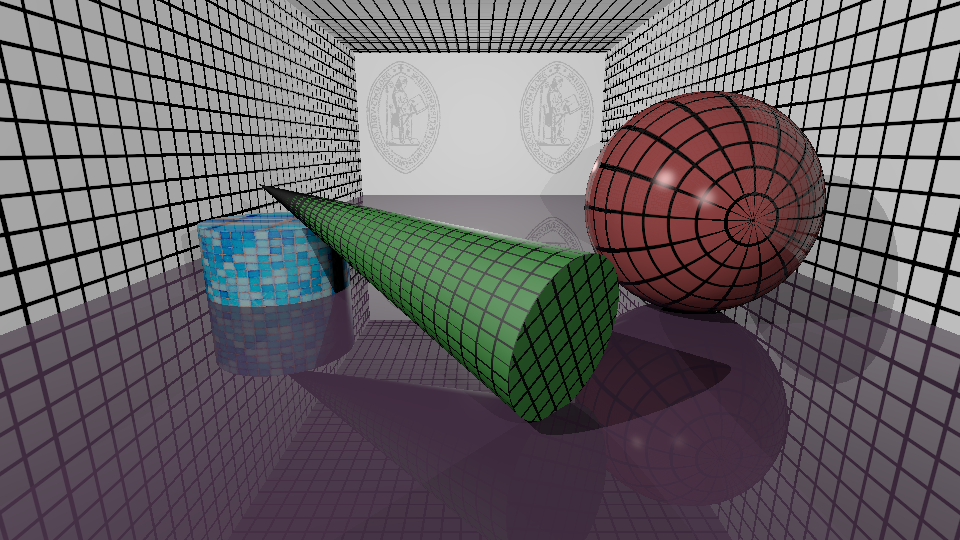
\includegraphics[width=13cm]{images/2-monimage.png}
		\caption{Image obtenue après le développement de \texttt{interpolateTexture()}}
		\label{fig:fig1}
	\end{figure}
	\section{Opérateur d'intégration pour le filtrage de texture}
	Une fois cette fonction développée, le temps d'exécution à grimpé en flèche comme le montre le listing \ref{lst:time1}.
	\begin{figure}[H]
		\centering
		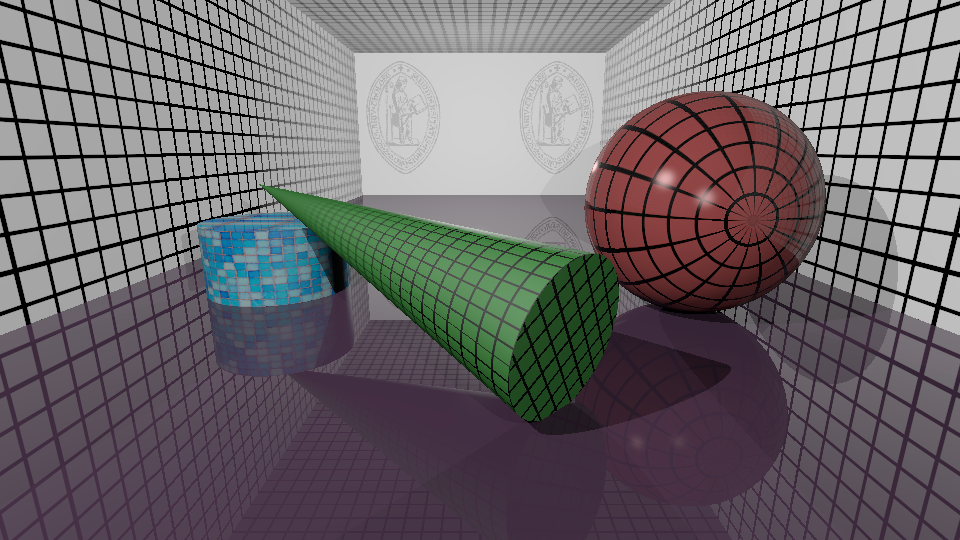
\includegraphics[width=13cm]{images/3-monimage.png}
		\caption{Image obtenue après le développement de \texttt{integrateTexture()}}
		\label{fig:fig1}
	\end{figure}
	Cette méthode, par les calculs d'interpolation, permet d'effectuer un dégradé de flou au fond de l'image. Le flou s'applique ainsi en fonction de
	la profondeur : plus on est loin du 1$^{er}$ plan, plus l'image sera flou, c'est ainsi que nous avons une meilleure impression de profondeur.

	\begin{lstlisting}[language=Sh, label=lst:time1, caption=Temps d'execution avec \texttt{interpolateTexture}]
aroquemaurel@Luffy ~/projets/cpp/raytracing/bin <master> time ./main
./main  18,92s user 0,03s system 99% cpu 19,010 total

\end{lstlisting}
Comme dit précédemment, cette méthode à l'inconvénient de ralentir considérablement le temps d'exécution. Cela vient des calculs nécessaires pour
cette interpolation, notamment un grand nombre de division.

\section{Opérateur de pré-filtrage de texture}\label{diminution}
	Cette fonction n'avait pas pour but d'améliorer l'image, mais uniquement de réduire le temps d'exécution. Cela a été un succès, après le développement de cette fonction, le temps d'exécution a été divisé par plus de 4 ! 
\begin{lstlisting}[language=Sh]
aroquemaurel@Luffy ~/projets/cpp/raytracing/bin <master> time ./main
./main  4,00s user 0,02s system 99% cpu 4,028 total
\end{lstlisting}

Grâce à cette méthode, nous avons réussi à atteindre un temps d'exécution convenable vis-à-vis de la qualité de l'image que nous avons obtenus comme
le montre la courbe figure \ref{fig:tpsCalcul}.
% 3.3992
% 4.028
% 18.92
% 4.9

\begin{figure}[H]
	\centering
	\begin{tikzpicture}[scale=.7]
		\begin{axis}[xtick={1,20,40,60},xlabel={\textbf{Fonction}}, 
			ylabel={\textbf{Tempx d'éxecution (s)}}, 
			xticklabels={\texttt{getTextel()}, \texttt{interpolateTexture()}, \texttt{integrateTexture()},\texttt{prefilterTexture()}}, width=18cm]
			\addplot coordinates{(1,3.3992)(20,4.028)(40,18.92)(60,4.9)};
		\end{axis}
	\end{tikzpicture}
	\caption{Temps d'exécution des techniques d'améliorations de l'image}
	\label{fig:tpsCalcul}
\end{figure}
	\begin{figure}[H]
		\centering
		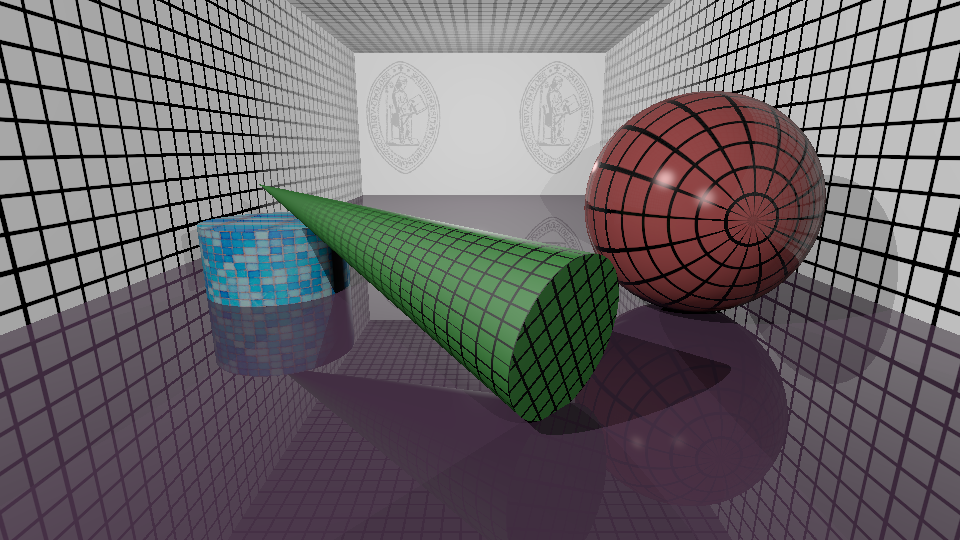
\includegraphics[width=13cm]{images/4-monimage.png}
		\caption{Image obtenue après le développement de \texttt{prefilterTexture()}}
		\label{fig:fig1}
	\end{figure}

	\section{Analyse et estimation des limites des techniques de filtrage implantées}
	La méthode que nous avons implémenté à permis d'améliorer considérablement l'image, ceci en créant des effets de flous et en lisant les effets de
	crénelage. 

	Cependant, cette méthode est loin d'être parfaite, en effet en premier lieu, il y a une perte d'information, notamment avec la moyenne des pixels
	voisins. Également, le temps d'exécution est assez important, et très gourmand en ressource, particulièrement pour de grandes images en HD. Ce
	temps de calcul a été diminué grâce à la section \ref{diminution}, mais cela reste assez important.



\end{document}
